\documentclass[a4paper,twoside]{article}

%for russian text
\usepackage[utf8]{inputenc}
\usepackage[english,russian]{babel}

%for images
\usepackage{graphicx}
\graphicspath{ {./images/} }
\usepackage{wrapfig}


%for margins and page dimentions
\usepackage[top=2cm, bottom=3cm, left=3cm, right=2.5cm]{geometry}
\usepackage{fancyhdr}
\renewcommand{\headrulewidth}{0pt}
\pagestyle{fancyplain}

%for table
\usepackage{array}

%for columns
\usepackage{multicol}
\setlength{\columnsep}{1cm}

%for spacing
\usepackage{setspace}

%headers and footers [odd]{even}
\lhead[]{}
\chead[]{}
\rhead[]{}
\lfoot[\textbf{62}]{}
\cfoot[]{}
\rfoot[]{\textbf{61}}


\begin{document}
\noindent\rule{16cm}{0.4pt}\vspace*{1cm}\\
\begin{wrapfigure}[3]{l}{0.15\textwidth}
\vspace*{-1.7cm}\hspace*{2cm}
\includegraphics[width=0.15\textwidth]{l}
\end{wrapfigure}
\hspace*{1.5cm}\Huge\textbf{ Правильная пирамида}\\
\newline\vspace*{1cm}
\hspace*{1.5cm}\normalsize\textit{В. К. Егерев, А. Г. Мордкович}\\
\noindent\rule{16cm}{0.4pt}\\
\vspace*{-0.7cm}

\begin{spacing}{1.1}
\begin{large}
\begin{multicols*}{2}
\noindent Решению многих геометрических задач присущ характер искусственности, что дало основание немецкому философу прошлого века Артуру Шопенгауэру бросить геометрии упрек в использовании «доказательств-мышеловок». Действительно, решение геометрических задач содержит мало шаблонов и часто производит впечатление фокуса. Тем более важно знать тот небольшой арсенал «стандартных» приемов, которые все-таки используются при решении этих задач. О некоторых приемах уже шла речь на страницах нашего журнала (см. например, статью И. А. Кушнир «Метод вспомогательного элемента», «Квант», 1974, № 2). В этой статье рассказывается еще об одном таком приеме.\\


\noindent\textbf{1. «Метод кастрюльки»}\\
Начнем с небольшой притчи. Андрею объяснили, как сварить яйцо: «Сними с гвоздя кастрюльку, налей туда воды, положи яйцо, зажги газ, поставь кастрюльку на газовую плиту и сними через 5 минут после того, как закипит вода». Андрюша так и сделал, все хорошо получилось. Но как-то, проснувшись утром, Андрей увидел, что вода в кастрюльку уже налита и газ горит. Подумав, он погасил газ, вылил воду и повесил кастрюльку на гвоздик, а затем сделал так, как его учили.\\
\indent Несмотря на кажущуюся несуразность такого поведения, метод возвращения к исходным данным задачи, которую мы умеем решать, является иногда наиболее рациональным. Назовем его «методом кастрюльки».\\

\noindent\textbf{2. Соотношения между углами в пирамиде}\\
На рисунке 1 изображена часть правильной п-угольной пирамиды SABCD…, SH-высота, SK-апофема. Введем следующие обозначения:

\leftskip=0.5cm
\noindent$\alpha$-угол между боковым ребром и плоскостью основания;\\
$\beta$-угол между боковой гранью и плоскостью основания;\\
$\gamma$-угол между смежными боковыми ребрами;\\
$\varphi$-угол между смежными боковыми гранями.

\leftskip=0cm
\vspace*{0.5cm}
\noindent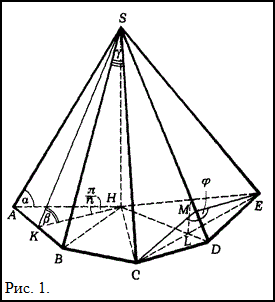
\includegraphics{fig1}
\end{multicols*}
\end{large}
\end{spacing}

\hspace*{-5ex}
\begin{tabular}{ c | c r| c | c }
\hline
Углы & \hspace*{0.7cm} Соотношения&& Область изменения углов & Связи между углами\\
\hline
&&&\\
$\alpha: \varphi$ & $\displaystyle \sin \alpha = \cot \frac{\varphi}{2} \cot \frac{\pi}{n}$ & (1)& $\displaystyle 0 < \alpha < \frac{\pi}{2}$ & \\
&&&\\
$\alpha: \gamma$ & $\displaystyle \cos \alpha = \sin \frac{\gamma}{2}/\sin \frac{\pi}{n}$ & (2)& $\displaystyle 0 < \beta < \frac{\pi}{2}$ & $\displaystyle \gamma < \pi - 2\alpha$ \\
&&&\\
$\alpha: \beta$ & $\displaystyle \tan \alpha = \tan \beta \cdot \cos \frac{\pi}{n}$ & (3)& $\displaystyle 0 < \gamma < \frac{\pi}{2}$ & $\displaystyle \alpha< \beta$ \\
&&&\\
$\beta: \gamma$ & $\displaystyle \cos \beta = \tan \frac{\gamma}{2}/\cot\frac{\pi}{n}$ & (4)& $\displaystyle \pi - \frac{2\pi}{n} < \varphi < \ \pi$ & \\
&&&\\
$\beta: \varphi$ & $\displaystyle \tan \beta = \frac {\sqrt{2} \cos \frac{\varphi}{2} } {\sqrt{-\cos \varphi - \cos \frac{2\pi}{n} } }$ & (5)& & $\displaystyle \varphi > \pi - 2\beta$ \\
&&&\\
$\gamma: \varphi$ & $\displaystyle \sin \frac{\gamma}{2} = \frac {\sqrt{-\cos \varphi - \cos \frac{2\pi}{n}}} {\sqrt{2} \cos \frac{\varphi}{2}}$ & (6)& & \\
\end{tabular}

\end{document}